\documentclass[11pt]{article}
\renewcommand{\baselinestretch}{1.05}
\usepackage[spanish]{babel}
\usepackage[utf8]{inputenc}
\usepackage{lipsum}

\usepackage{amsmath,amsthm,verbatim,amssymb,amsfonts,amscd}
\usepackage{graphicx, wrapfig}
\usepackage{float}
\usepackage{caption, subcaption}
\usepackage{tkz-fct}
\usetikzlibrary{babel}
\usepackage{pgfplots}
\usepackage{enumitem}
\usepackage{multicol, vwcol}
\usepackage{listingsutf8}
\usepackage{color}
\usepackage{hyperref}
\usepackage{booktabs}
\usepackage{ marvosym }
\usepackage[sorting=none]{biblatex}
\bibliography{bibliography.bib}
\definecolor{lightgray}{gray}{0.95}

\hypersetup{
    bookmarks=true,         % show bookmarks bar?
    unicode=false,          % non-Latin characters in Acrobat’s bookmarks
    pdftoolbar=true,        % show Acrobat’s toolbar?
    pdfmenubar=true,        % show Acrobat’s menu?
    pdffitwindow=false,     % window fit to page when opened
    pdfstartview={FitW},    % fits the width of the page to the window
    pdftitle={Ingeniería, empresa y sociedad - Entrega 2},    % title
    pdfauthor={Francisco Luque, María del Mar Ruiz},     % author
    pdfsubject={Ingeniería, Empresa y Sociedad},   % subject of the document
    pdfnewwindow=true,      % links in new PDF window
    colorlinks=true,        % false: boxed links; true: colored links
    linkcolor=red,          % color of internal links (change box color with linkbordercolor)
    citecolor=cyan,         % color of links to bibliography
    filecolor=magenta,      % color of file links
    urlcolor=blue           % color of external links
}

\topmargin0.0cm
\headheight0.0cm
\headsep0.0cm
\oddsidemargin0.0cm
\textheight23.0cm
\textwidth16.5cm
\footskip1.0cm
\theoremstyle{plain}

\newtheorem{theorem}{Teorema}
\newtheorem{corollary}{Corolario}
\newtheorem{lemma}{Lema}
\newtheorem{proposition}{Proposición}
\theoremstyle{definition}
\newtheorem{definition}{Definición}
\newtheorem{example}{Ejemplo}

\newcommand{\N}{\mathbb{N}}
\newcommand{\Z}{\mathbb{Z}}
\newcommand{\Q}{\mathbb{Q}}
\newcommand{\C}{\mathbb{C}}
\newcommand{\R}{\mathbb{R}}

\begin{document}

\title{Ingeniería, Empresa y Sociedad \\
  DGIIM \\
  \large Estructura de propiedad, gobierno corporativo y
  responsabilidad social corporativa de Inditex}
\author{Francisco Luque Sánchez\\
  María del Mar Ruiz Martín}
\maketitle

En este caso práctico se desarrollará un informe sobre las
características de la empresa INDITEX \cite{inditex}. En primer lugar,
se comentarán algunas características generales de la misma,
utilizando para ello la información que se muestra en su página web,
así como los informes que nos han sido entregados. A continuación,
comentaremos brevemente su gobierno corporativo, la estructura de
propiedad, y su responsabilidad social corporativa.\\

Comenzamos describiendo algunas características de la empresa.

\section*{Apartado 1: Descripción de la empresa}

INDITEX (acrónimo de Industria de diseño textil) es un grupo
multinacional español fundado en el año 1985. Su sector de actividad
es la industria manufacturera, concretamente la industria
textil. Actualmente cuenta con más de 162000 empleados en todo el
mundo, repartidos en más de 7500 tiendas. A este número hay que
sumarle las más de 3700 fábricas repartidas también por todo el
territorio mundial.\\

En cuanto a los mercados en los que tiene localizada su actividad de
producción, cabe destacar Europa, donde tienen más de 5000 tiendas. A
continuación, aparece América, donde se encuentran aproximadamente 800
tiendas, teniendo situadas las demás por el resto del mundo. No
comentamos nada sobre la localización de sus plantas de producción ya
que en la página web no hemos sido capaces de localizar ese dato. Se
comenta brevemente que su actividad económica se centra básicamente en
Arteixo, un pueblo de A Coruña donde INDITEX tiene su sede. Aparece
que más de la mitad de las fábricas del grupo no están situadas ni en
Europa ni en América, pero no se especifica en qué parte del mundo se
encuentran las mismas. Además, no se especifica si con América se
refieren exclusivamente a América del Norte o se incluye también
Centroamérica y
América del Sur.\\

Atendiendo al volumen de negocio, según los datos de la página web, en
2016 (último dato que se ofrece, no está disponible todavía el dato de
2017) se facturaron en ventas 23311 millones de euros. En cuanto al
beneficio bruto, ese año se consiguieron 5083 millones de euros, que
tras el pago de impuestos y tasas se convierten en 3157 millones.
Además, cabe destacar que desde el año 2008, año en el que comienzan
los registros que se muestran en la página web, la empresa ha
conseguido siempre un mayor nivel de ingresos que el año
anterior. Concretamente, desde el año 2008 se han duplicado las
ganancias anuales de la empresa.\\

Pasamos a comentar ahora la información que la empresa ofrece sobre su
gobierno corporativo en la página web.

\section*{Apartado 2: Información sobre el gobierno corporativo en la
  página web}

En la página web de la empresa aparece un apartado bastante extenso
dedicado exclusivamente al gobierno corporativo de la misma. Tras
entrar a este apartado, lo primero que se muestra es información sobre
la Junta General de accionistas \cite{corp-gov}. Nos permiten
descargar públicamente el reglamento de la junta, y se nos muestran
enlaces para acceder al foro electrónico, así como a la plataforma de
voto. Creemos que en una empresa de tal tamaño es importante aportar a
los accionistas estas herramientas, ya que permiten la interconexión
entre todos ellos, a pesar de encontrarse la mayoría en distintos
puntos del mundo.\\

Más adelante encontramos información sobre el consejo de
administración, donde podemos encontrar los miembros que lo fundan,
así como distintos reglamentos (del consejo, de la comisión de
nombramientos, de auditoría...).\\

Tenemos también a nuestra disposición los informes anuales del
gobierno corporativo desde el año 2011 hasta 2016, así como informes
de remuneración, reglamentos de conducta para los integrantes
del gobierno corporativo, y los estatutos de la fundación.\\

Como podemos observar, la empresa tiene un gran interés en mostrar de
forma pública toda su actividad, a fin de ganar la confianza de los
inversores. Una política de transparencia e información por parte de
la empresa suele ser un reclamo importante para los accionistas, ya
que pueden conocer con relativa facilidad el funcionamiento y
gobierno de la empresa en la que tienen acciones.\\

Vamos a comentar brevemente los epígrafes que aparecen en el informe
anual de gobierno corporativo del año 2016, que es el último
disponible.  En la página web aparece un anuncio informando de que los
resultados de la empresa para el año 2017 se harán públicos el día 14
de marzo, por lo que no los tenemos disponibles en el momento de
redactar este
caso práctico.\\

En el informe mencionado aparecen los siguientes apartados (además del
PDF descargable desde la página web, tenemos disponible una web en la
que se hace un repaso del ejercicio económico anual
\cite{annual-report}):

\begin{description}
\item[A] Estructura de la propiedad
\item[B] Junta general
\item[C] Estructura de administración de la sociedad
\item[D] Operaciones vinculadas y operaciones intragrupo
\item[E] Sistemas de control de riesgo
\item[F] SCIIF
\item[G] Grado de seguimiento de las recomendaciones de gobierno
  corporativo
\item[H] Otra información de interés
\end{description}

No comentamos en profundidad estos apartados ya que el informe es muy
extenso (cuenta con más de 100 páginas). No obstante, hemos podido
observar que INDITEX se toma muy en serio la imagen de la empresa,
y facilitan toda la información posible a su público.\\

Pasamos a comentar ahora la estructura de propiedad de la empresa,
utilizando para ello los archivos que se nos han facilitado.

\section*{Apartado 3: Estructura de propiedad de la empresa}

Para desarrollar este apartado, trataremos de analizar la estructura
de propiedad que presenta INDITEX. Para esto nos centraremos en los
datos aportados en el archivo ``ownership''.\\

En primer lugar analizaremos la distribución de las acciones de la
empresa.  Para ello, en la siguiente gráfica mostraremos el porcentaje
de acciones en circulación que poseen los 20 primeros accionistas:

\begin{figure}[H]
  \centering
  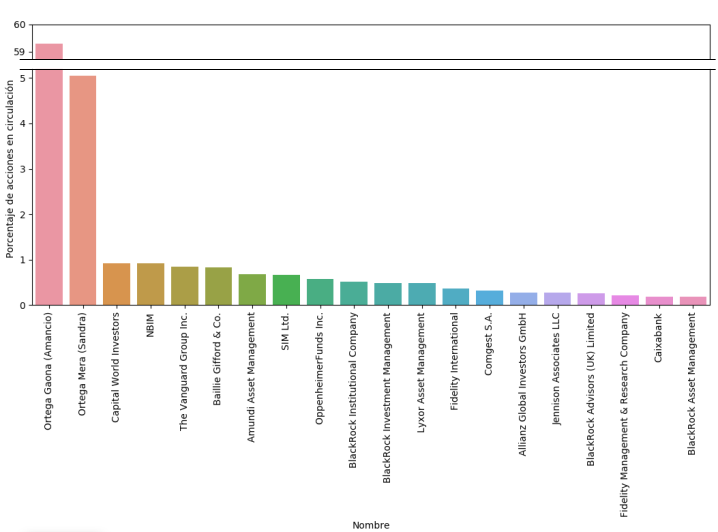
\includegraphics[width=.85\textwidth]{graphs/barplot_finished.png}
  \caption{Distribución de las acciones de INDITEX}
\end{figure}


En el gráfico podemos ver que Amancio Ortega es el accionista
mayoritario, poseyendo el 59.29\% de las acciones. Además, su hija,
Sandra Ortega, cuenta con algo más del 5\% de las acciones, lo que la
convierte en la número dos del ranking de accionistas. Por tanto, casi
un 65\% de la empresa
queda en manos de la familia Ortega.\\

El resto de accionistas contarán con menos de un 1\% de las acciones
cada uno, lo cual supone un gran salto de la posición dos a la tres,
tal y como se observa en el gráfico. Entre estos otros accionistas se
puede destacar Capital World Investors, Norges Bank Investment
Management o The Vanguard Group. Resulta además remarcable que Amancio
y Sandra, además de los dos primeros accionistas, son los
únicos accionistas del top 20 que no son empresas.\\


Para continuar con el estudio de la propiedad de INDITEX, vamos a
examinar la distribución de los inversores en los diferentes
países. Podemos ver dicha información representada a continuación:

\begin{figure}[H]
  \centering 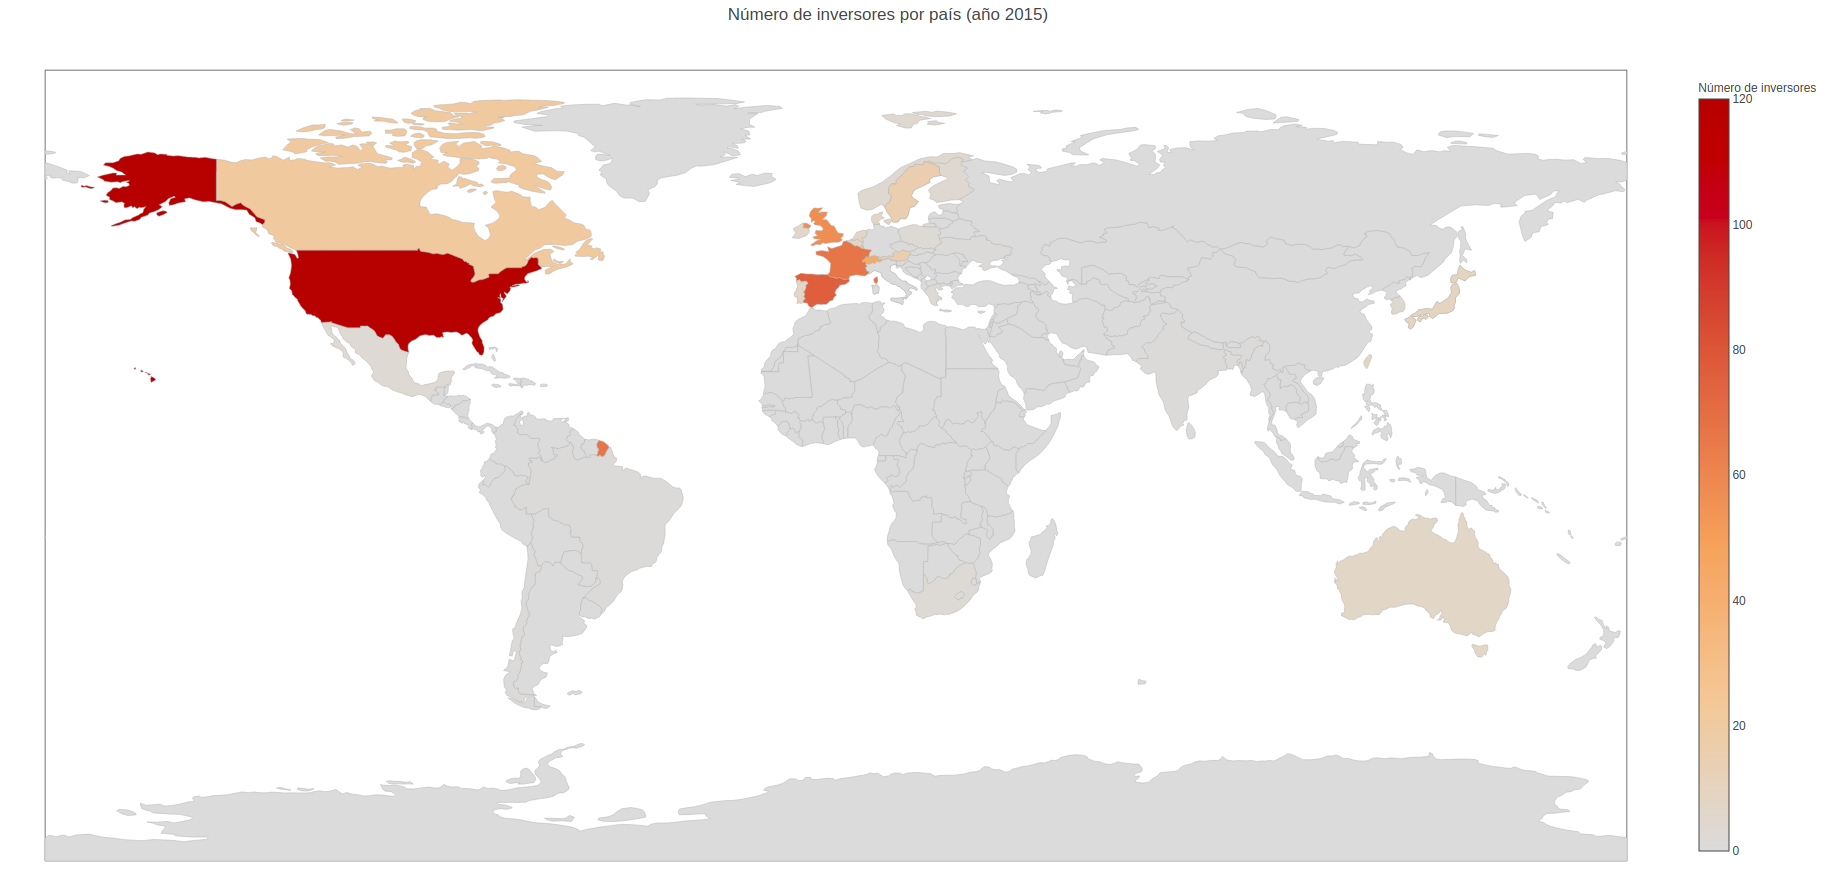
\includegraphics[width=\textwidth]{graphs/worldmap.png}
  \caption{Distribución de los accionistas de INDITEX}
\end{figure}


Observamos que la mayoría de los accionistas son procedentes de
Estados Unidos.  Concretamente 120 de los 620 inversores son de
Estados Unidos. A continuación encontramos a España, con un total de
76 inversores. Ésta será seguida de Francia, Alemania y Reino Unido
con un total de 67, 59 y 57 inversores respectivamente. Por tanto,
aunque el país con mayor número de accionistas sea Estados Unidos,
podemos destacar que la mayoría de los mismos son residentes
europeos, suponiendo estos más de un tercio de los accionistas totales.\\


En el resto de continentes encontramos pocos inversores. En el
continente asiático encontramos inversores en Japón, Hong Kong o
Taiwan. En Oceanía hay presentes accionistas tan solo en
Australia. Finalmente, de Sudamérica y Centro América podemos
nombrar a México, Chile y Brasil.\\

Finalmente vamos a mostrar un gráfico con información sobre el tráfico
de acciones.  Para ello veremos el porcentaje de acciones que se han
vendido, comprado o mantenido.


\begin{figure}[H]
  \centering 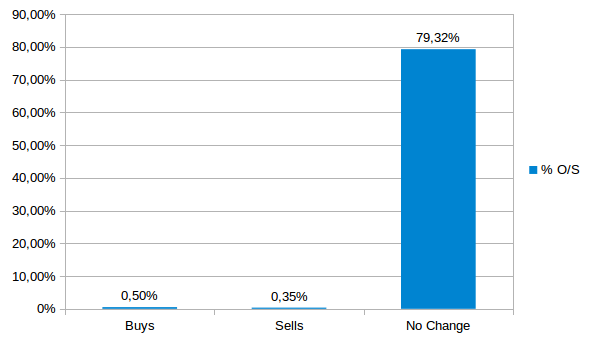
\includegraphics[width=\textwidth]{graphs/rotations.png}
  \caption{Tráfico de las acciones de INDITEX}
\end{figure}

De la imagen anterior podemos afirmar que la propiedad de las acciones
de la empresa es muy estable, ya que se ha mantenido el 79.32\% de las
acciones totales, mientras que el tránsito de acciones se compone tan
solo de un 0.5\% de compras y un 0.35\%
de ventas.\\

Finalmente vamos a mostrar algunos gráficos que permitan observar la
responsabilidad social corporativa y el gobierno corporativo de la
empresa.

\section*{Apartado 4: Gobierno corporativo y responsabilidad social
  corporativa}

En este apartado vamos a mostrar tres gráficos que nos van a permitir
conocer parte de la responsabilidad social corporativa de la
empresa. Empezaremos con su responsabilidad medioambiental. En el
gráfico siguiente se muestra el uso de energía, agua y emisiones de
$CO_2$ que produce la empresa por cada millón de dólares que genera en
ingresos:

\begin{figure}[H]
  \centering
  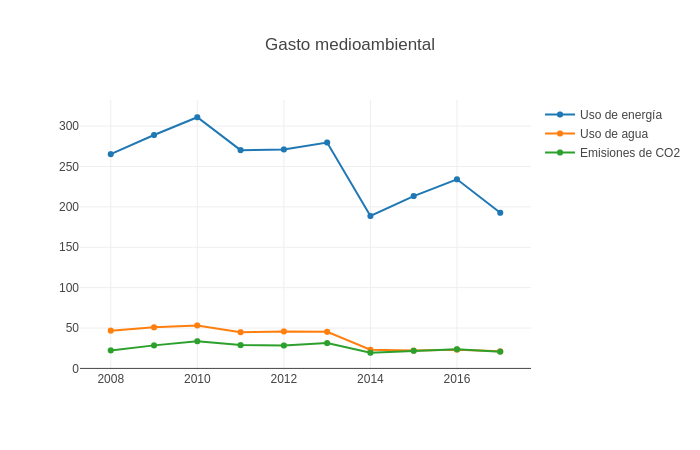
\includegraphics[width=\textwidth]{graphs/environment.png}
  \caption{Gasto medioambiental de INDITEX}
\end{figure}

Podemos observar que en los últimos años se ha conseguido una
reducción sensible del gasto en todos los sentidos. Cabe destacar que
el mayor consumo que se produce es en energía. No obstante, tanto en el
uso de recursos como en las emisiones producidas la empresa obtiene la
puntuación más alta posible. Concretamente, desde que se tiene
registro, excepto el primer año, consiguen la mejor puntuación en
cuanto a emisiones (en 2008 consiguieron A, que es la segunda mejor),
y en cuanto a consumo han conseguido la puntuación más alta durante
los dos últimos años. Esto nos hace pensar que en este apartado la
empresa hace un importante esfuerzo para conseguir unos resultados
excelentes. Pasamos a comentar la responsabilidad social de la empresa.\\

En el gráfico que se muestra a continuación se resume información
sobre el papel de las mujeres en esta empresa:

\begin{figure}[H]
  \centering 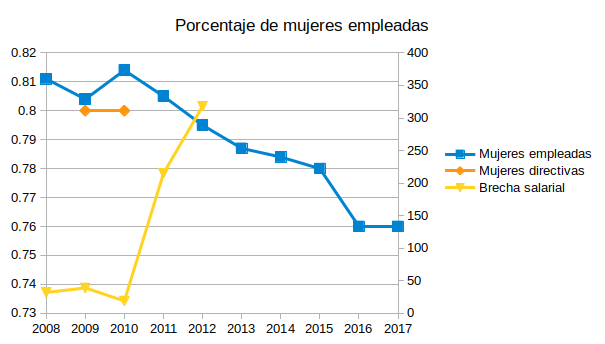
\includegraphics[width=\textwidth]{graphs/social.png}
  \caption{Gasto medioambiental de INDITEX}
\end{figure}

Podemos obervar varios comportamientos interesantes en este gráfico.
Se muestran tres líneas distintas. Comenzaremos comentando la línea
azul, que muestra el porcentaje de mujeres que trabajan en la empresa
respecto del total de empleados. Resulta curioso observar que más del
80\% de la plantilla estaba constituida por mujeres en 2008, y aunque
este valor ha ido disminuyendo progresivamente desde ese año,
actualmente más de tres cuartas partes de los empleados siguen siendo
mujeres. No es del todo sorprendente este hecho, ya que si pensamos en
las tiendas de ropa de esta cadena, podemos recordar que
la mayoría de dependientes de las mismas son mujeres.\\

Las otras dos líneas sí que presentan comportamientos más
sorprendentes. Comenzamos con la línea naranja. Esta línea muestra el
porcentaje de personas del equipo directivo que son mujeres. Lo más
destacable de este dato es que sólo se nos aportan dos registros, del
año 2009 y el año 2010, aunque ciertamente son bastante altos (80 \%).
Lo más destacable de esta línea nos lleva a compararla con la tercera
mostrada. En dicha línea se muestra la brecha salarial de la empresa.
Justo en el año en el que se deja de tener registro del porcentaje de
mujeres directivas comienza a dispararse la brecha salarial en la
empresa. También resulta impresionante observar cómo aumenta la brecha
salarial durante dos años consecutivos, aumentando la misma en casi
300 puntos, y a partir de ahí dejan de tenerse registros de dicho
dato. Se puede deducir de este gráfico que no parece que la empresa
tenga un comportamiento especial en la búsqueda de la igualdad entre
sus trabajadores, un comportamiento que puede ser reprochable. Además,
cabe destacar que en la página web de INDITEX, en el apartado del
consejo de administración, sólo uno de los 9 perfiles que aparecen
listados pertenece a una mujer.\\

Pasamos a comentar datos sobre el gobierno corporativo de la empresa.

\printbibliography

\end{document}
